% !TEX root = ../thesis.tex
\chapter{基于相似性学习的移动端实时抠图方法}
\section{引言}
上一章中提出了基于相似性学习的信息传播在一般性的图像抠图任务上的应用方法,在本章中我们将研究如何将引导滤波器的思想方法结合到神经网络中,以达到近似引导上下文注意力机制的效果,实现移动端的高效实时抠图。

图像抠图任务的提出不仅仅是为了进行高精度的图像分割,更是为了对自然图像进行合理地分解,因为抠图任务同时需要考虑物体的透明度。抠图算法生成的alpha遮罩可以大大减少广告、设计、电影等行业中对图像或视频进行编辑的工作量以及技能要求。
随着在移动设备上编辑图像或视频的用户数量快速增长,高效、准确且能提升用户体验的自然图像抠图算法已成为一个重要的需求。

目前在移动设备上进行图像抠图存在两个难点。一方面,因为图像抠图是对高分辨率alpha遮罩进行估计的计算密集型任务,目前绝大多数抠图方法\cite{levin2008closed,chen2013knn,cho2016natural,xu2017deep}无法在移动设备上实现实时处理。另一方面,多数现有的抠图方法对输入的trimap图的质量十分敏感。虽然有部分基于涂抹(scribble-based)\cite{lee2011nonlocal}和交互式\cite{yang2018active}的抠图方法在近几年被提出,但是不正确的涂抹或输入信息依然会导致具有复杂纹理的图像的抠图结果存在大量错误。

通常情况下,由于时间延迟和计算能力的限制,我们只能在移动设备上获得弱标注分割掩码。我们通过弱标注分割掩码(weakly annotated mask)这个词来描述一个存在噪声或不完全正确的分割掩码,改掩码可以对图像上的前景和背景提供一个近似准确的标注信息。这里对弱标注的定义与弱监督分割\cite{papandreou2015weakly}或定位\cite{oquab2015object}中的弱标注略有区别。
弱标注分割掩码可以是分割方法所输出的二进制图像、阈值化后的深度图或是来自用户交互的不准确的掩码标注。它与传统的trimap图不同,传统的trimap图是绝对正确的,但需要更多的人工标注时间。
  换句话说,传统的trimap图中要求不存在将前景区域标注为背景的错误情况,或是将部分背景像素标注为前景的错误。大多数传统的图像抠图方法都将输入的trimap图视为完全正确的指导标准,仅在标注的未知区域中计算alpha遮罩值。尽管弱标注分割掩码意味着在输入的掩码中会存在此类标注错误,但是如果该掩码是通过分割方法自动生成的,则此类错误往往无法避免。同时,降低输入trimap图或掩码的标注质量可能会严重影响传统抠图方法的性能。

先验信息作为对可行域的一个约束,已经在一些先前的工作中被深入研究,以改进图像生成类任务\cite{ulyanov2018deep}。
在图像抠图任务中,适当设计alpha遮罩的先验可以在图像抠图中增加解空间约束同时降低计算需求。
在本章所提出的方法中,我们重新思考了不同手工设计的抠图算法中所隐含的alpha遮罩先验,并意识到引导滤波器(guided filter)\cite{he2010guided}中的保梯度先验(gradient preserving prior)可以被无缝集成到深度神经网络中。
本章提出了一种专为移动设备设计的深度图像抠图框架,命名为归纳引导滤波器(Inductive Guided Filter,IGF),该框架在保持了可用精度同时大幅减少网络参数和计算时间。与高度依赖trimap图质量的经典方法相比,本章提出的IGF模型对弱标注分割掩码输入具有鲁棒性。我们参考图像翻译(image-to-image translation)的形式建立了该深度神经网络。
借助生成对抗网络(Generative Adversarial Networks,GAN)框架以及三个不同的训练损失函数,所提出的方法可以仅使用一个极小的神经网络生成出具有详细纹理细节的alpha遮罩。
在给定一个分割模型作为所提出的归纳引导滤波器的预处理器的情况下,可以构建出一条从输入图像到alpha遮罩的全自动语义抠图流水线,而无需人工干预。
所提出的IGF方法有助于自然图像抠图在无限制的环境中特别是在移动设备上具有更强的实用性。

\section{相关工作}
在本节中,我们将对与本章相关性较强的部分深度图像抠图方法及引导滤波器相关方法进行简单回顾。

根据应用场景的不同,深度图像抠图算法可以大致分为两类:通用深度图像抠图方法和为特定应用设计的专用抠图方法。
通用深度图像抠图方法以理想化的trimap图作为输入信息,以对自然图像的alpha遮罩进行预测,例如第五章中所介绍到的\parencite{cho2019deep,xu2017deep,lutz2018alphagan,cai2019disentangled,lu2019indices,hou2019context,samplenet}等,该类方法严重依赖trimap作为输入,以减小解空间。然而近几年,对于特定的实际问题,一些方法通过利用图像语义信息可以在没有任何trimap图输入的情况下取得良好的抠图效果。
Shen等人\cite{shen2016deep}将端到端卷积神经网络与Closed-form Matting\cite{levin2008closed}结合起来,自动生成人像(portrait)图片的trimap图,然后获得所需的alpha遮罩值。值得注意的是,在文献\parencite{shen2016deep}所提出的方法使用了一个统计上的前景概率图作为输入,该概率图在形式上看似与IGF方法中所使用分割掩码输入相同,但事实两者上存在很大的区别。文献\parencite{shen2016deep}中所用的前景概率图为一个固定的先验图,对任意输入图片都采用同一个先验概率图,且该方法为语义抠图而非通用抠图方法。
Chen等人\cite{chen2018semantic}提出了一种语义人体抠图(Semantic Human Matting,SHM)方法,将语义分割网络与抠图网络集成在一起,在网络中间预测trimap图,以自动提取人体的alpha遮罩。后续有多篇文献\cite{zhu2017fast,levinshtein2018real,chen2019boundary}提出了可以在移动设备上对人像或头发进行语义抠图或精细化分割的轻量级模型。

He等人在文献\parencite{he2010guided}中提出了引导滤波器,引导滤波器可以看作一个具有保边缘(edge-preserving)能力的平滑算子,并且与抠图中常用的拉普拉斯矩阵具有理论上的联系。
深度引导滤波器(Deep Guided Filter,DGF)\cite{wu2018fast} 将引导滤波器作用于图像翻译模型的输出图像,作为一个超分辨率模块,并且将最终的损失函数梯度经过引导滤波器反向传播回低分辨率输入图像。Zhu等人在文献\parencite{zhu2017fast}中受引导滤波器启发,提出了一个带有羽化模块(feathering block)的快速人像抠图方法,在第\ref{sec6:igf}中我们将对该方法进行详细说明与比较。

\begin{figure}[t]
	\centering
	\includegraphics[width = 0.75\columnwidth]{chap6/archtecture.pdf}
	\bicaption{所提出架构示意图}{An illustration of our architecture}
	\label{fig6:archtecture}
\end{figure}
\begin{figure}[t]
	\centering
	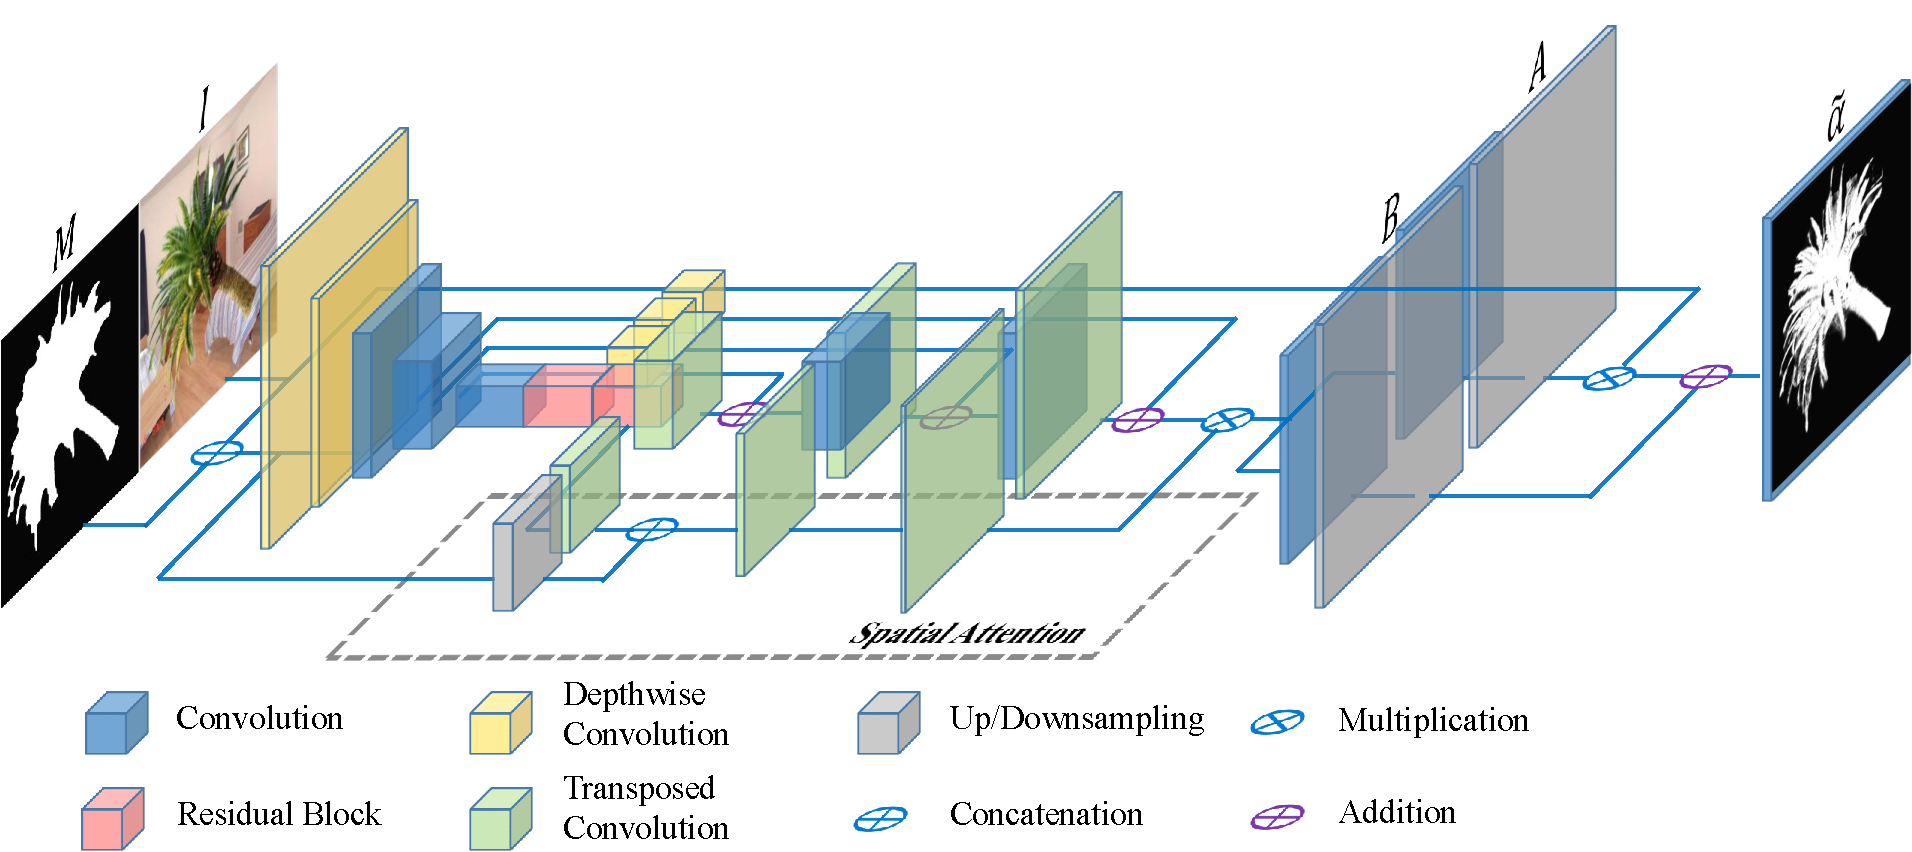
\includegraphics[width = 0.95\columnwidth]{chap6/generator.pdf}
	\bicaption{所提出生成器的概貌。线性系数$A$和$B$从共享相同主干网络的两个分支中生成。最右侧两个缩放系数为4的上采样层用于模仿快速引导滤波器\cite{he2015fast}以加快推理速度}{The overview of our generator. Linear coefficients $A$ and $B$ are generated from two branches sharing the same backbone. The right-most two upsampling layers both have a factor 4 which mimic Fast Guided Filter \cite{he2015fast} for acceleration
	}
	\label{fig6:generator}
\end{figure}

\section{归纳引导滤波器方法}
归纳引导滤波器方法将建立一个高效的、以弱标注分割掩码为输入的图像抠图网络模型。为此,我们采用了引导滤波器\cite{he2010guided}中的线性模型假设,而引导滤波器正由于其具有的保梯度先验,得以稳定且高效地实现其滤波器功能。
借鉴文献\parencite{lutz2018alphagan}的设计,我们在模型中采用生成对抗网络\cite{goodfellow2014generative}结构。图\ref{fig6:archtecture}中粗略说明了所提出方法的网络架构,图\ref{fig6:generator}中详细介绍了所提出的生成器。
\subsection{归纳引导滤波器的公式化}
在引导滤波器\cite{he2010guided}对于图像抠图问题的建模中的基本假设为,输出alpha遮罩图为引导图像$I$在中心点为像素$k$的邻域$\omega_k$内的线性变换:
\begin{equation}
\alpha_i = A_{k}I_{i} + B_{k}, \forall i \in \omega_k,
\end{equation}
其中$ A_{k} $ 和 $ B_{k} $为待优化的线性系数。该线性假设同样被用于Closed-form Matting\cite{levin2008closed}方法中。在弱标注掩码作为输入的情况下,引导滤波器中的优化目标为在对$A_{k}$进行$\ell_2$正则化下最小化输出$\alpha_i$与其在弱标注掩码$ M $上相对应的像素值$M_i$的平方误差。在图像抠图的设定下,引导滤波器对每对输入图像和分割掩码分别求解优化问题,以获得从输入图像$I$到尽可能相似于掩码$M$的预测值$\alpha$的线性变换。该线性变换要求了alpha遮罩图需要具有与输入图像近似相同的梯度方向,即$ \nabla \alpha_i=A_k \nabla I_i $。该等式可以被看作为隐含的保梯度先验。

尽管引导滤波器可以作为一种对具有弱标注输入的图像抠图任务的快速且有效的方法,但其受限于最优alpha遮罩与弱标注掩码之间的差异应充分小这一约束。 从经验上讲,来自语义分割方法或用户交互的分割掩码与真实标注的alpha遮罩值会有较大的差异。

不同于引导滤波器,本章所提出的方法通过监督学习任务而不是优化问题实现图像抠图。在所提出的方法中,我们仅引入了保梯度先验而舍弃了引导滤波器中的目标函数即alpha预测值与输入掩码之间的约束。该基于线性变换假设的归纳模型可以有效利用图像抠图数据集中的真实标注信息。我们将所提出的归纳引导滤波器公式化为:
\begin{equation}
\alpha = \phi_{A}(I, M)\circ I + \phi_{B}(I, M), 
\label{eq6:igf}
\end{equation}
式中$ \circ $ 表示哈达玛积(Hadamard product),且我们通过神经网络$ \phi_{A}(I, M) $ 和 $ \phi_{B}(I, M) $ 对引导滤波器中的$ A $ 和 $ B $ 进行参数化。网络 $ \phi_{A} $ 和 $ \phi_{B} $ 以原始图像 $ I $ 及分割掩码$ M $作为输入,共享网络主干参数(见图\ref{fig6:generator})。归纳引导滤波器方法的优化目标为最小化预测alpha值与真实标注值之间的alpha预测损失。

对于任意的输入图像和分割掩码,网络$ \phi_{A} $ 和$ \phi_{B} $ 可以生成特定的系数图$ A $ 及 $ B $,以构建出用于生成alpha遮罩估计的线性变换。 
由于 $ \phi_{A} $ 与 $ \phi_{B} $为卷积网络且最后一层为上采样层,从低分辨率特征图中经过上采样得到的$ A $ 和 $ B $,相对较为平滑。因此,线性变换系数图$ A $ 和 $ B $的梯度充分小,可以满足 $ \nabla \alpha \approx A \circ \nabla I $。
由于这一特性,所提出的网络结构可以内在地保持图像本身的梯度方向。

文献\parencite{zhu2017fast}中也提及了相似的思想方法。

\subsection{归纳引导滤波器中的相似性学习}

\subsection{生成器设计}
\subsection{判别器设计}

\section{实验结果}
\subsection{数据集}
\subsection{MAT-2793测试集实验结果}
\subsection{Composition-1k测试集实验结果}
\subsection{消融实验}
\subsection{效率评估实验结果}
\subsection{自然图像抠图效果}
\section{本章小结}